

%!TEX root = ../Notes.tex
\section{Hausdorffness} 
\begin{definition}
	Let $(X, F _X)$ be a topological space. We say that X is \textbf{Hausdorff} if $\forall$ $p, q \in X$ such that $p \neq q$, $\exists$ disjoint sets $U, V \in F_X$ such that $p \in U$, $q \in V$. 
\end{definition}
\begin{example}
	Metric spaces \textbf{are} Hausdorff. 
\end{example}
\begin{example}
	[a non-example] Any space containing at least two points under the indiscrete topology is \textbf{not} Hausdorff. 
\end{example}

Hausdorff is important because any ``reasonable'' space/any space that we want to be in will be Hausdorff.

\textbf{Note:} Continuous functions \emph{may not} preserve Hausdorff-ness. 
\begin{example}
	Define $f\colon(\R,\text{ discrete})\to (\R,\text{ indiscrete})$ by the identity map. 
\end{example}

This is continuous because the domain has the discrete topology, but the domain is Hausdorff while the range clearly is not. 
\begin{smallfact}
	Suppose $f \colon (X, F_X)$ $\to$ $(Y, F_Y)$ is a homeomorphism and $(X, F_X)$ is Hausdorff. Then $(Y, F_Y)$ is also Hausdorff. 
\end{smallfact}
\begin{proof}
	Let $p \neq q \in Y$. Because f is a bijection, $f^{-1}(p)$ and $f^{-1}(q)$ are distinct points in X.
	
	Since $X$ is Hausdorff, $\exists$ $U, V \in F_X$ such that $U \cap V = \emptyset$, $f^{-1}(p) \in U$, $f^{-1}(q) \in V$.
	
	Consider $f(U)$, $f(V)$. Since $f$ is a homeomorphism and, thus, open, $f(U)$ and $f(V)$ are open. Then, because $f$ is a bijection, we have $p \in$ $f(U)$, $q \in$ $f(V)$, and $f(U) \cap f(V)$ = $\emptyset$ 
\end{proof}

We are now interested in how Hausdorff-ness and compactness are related.\\

\textbf{Flapan Says...} `` Hausdorff-ness and compactness are like two people who love each other, because when two people love each other, they can do so much more together than they can alone.'' \\
\begin{theorem}
	Let $(X, F_X)$ be Hausdorff. Let A $\subseteq$ X be compact. Then A is closed. 
\end{theorem}
\begin{proof}
	(Compare the following to the proof that all compact subsets of metric spaces are closed. That is, we are going to show that we don't need a metric, just Hausdorff-ness, for closed subsets to be compact.)
	
	Rather than show $A$ is closed, we will show $X-A$ is open.
	
	Let $p \in X-A$. We want to show $\exists$ $U \in F_X$ such that $p \in U \subseteq X\setminus A$. Let $a \in A$. Because X is Hausdorff, $\exists$ $U_a, V_a \in F_X$ such that $p \in U_a$, $a \in V_a$, $U_a \cap V_a = \emptyset$.
	
	Consider $\{ V_a | a \in A\}$. This is an open cover of A because $V_a$ open and $a \in V_a$ $\forall a \in A$. So, because A is compact, $\exists$ finite subcover $\{ V_{a_1}, V_{a_2}, ..., V_{a_n}\}$
	
	Let $U = \bigcap_{i=1}^{n} U_{a_i}$. $U \in F_X$ since it is a finite intersection of elements of $F_X$ and $p \in U$ since $p \in U_{a_i}$ $\forall$ $i=1, 2, ...,$ $n$.
	
	\textbf{Claim:} $U \subseteq X-A$\\
	\emph{Proof.} $\forall$ $i=1, 2, ...$ $n$, we have $U_{a_i} \cap V_{a_i} = \emptyset$. Also, $A \subseteq \bigcup_{i=1}^{n} V_{a_i}$ and $U \cap A$ $\subseteq$ $U \cap \bigcup_{i=1}^{n} V_{a_i}$.
	
	However, $U \cap \bigcup_{i=1}^{n} V_{a_i} = \emptyset$ because if $\exists$ $x \in U \cap \bigcup_{i=1}^{n} V_{a_i}$, then $\exists$ $i_o$ such that $x \in V_{a_{i_o}} \cap U_{a_{i_o}}$. But, by definition, $V_{a_{i_o}} \cap U_{a_{i_o}} = \emptyset$, so no such $x$ exists. Thus,
	
	\[U \cap A\subseteq U \cap \bigcup_{i=1}^{n} V_{a_i} = \emptyset,\]
	meaning $U \cap A = \emptyset$. So, because $U \subseteq X$ but $U \cap A = \emptyset$, $U \subseteq X-A$
	
	Thus, we have found $U \in F_X$ such that $p \in U$, $U \subseteq X-A$. Thus, $X-A$ is open. Thus, \textbf{A is closed}. 
\end{proof}
\begin{corollary}
	In any Hausdorff space, (finite sets of) points are closed sets. 
\end{corollary}
\begin{proof}
	Let $p \in (X, F_X)$ and let $(X, F_X)$ be Hausdorff. Let $\{ U_i|i \in I\}$ be an open cover of $\{ p\}$. Then $\exists$ $i_o \in I$ such that $p \in U_{i_o}$. Thus $\{ U_{i_o} \}$ is a finite subcover. Hence, $\{ p \}$ is compact.
	
	Thus, by Theorem above, $\{ p\}$ is closed. 
\end{proof}
\begin{lemma}
	[it's \textbf{important!}] Let $f : (X, F_X) \to (Y, F_Y)$ be continuous. Let $X$ be compact, and $Y$ be Hausdorff. Then $f$ is a homeomorphism if and only if it is a bijection. 
\end{lemma}
\begin{proof}
	\begin{itemize}
		\item[($\Rightarrow$)] Since $f$ is a homeomorphism, $f$ is a bijection. 
		\item[($\Leftarrow$)] Suppose $f$ is a continuous bijection. We want to show that $f$ is open. Since $f$ is a bijection, this is equivalent to showing that $f$ is closed.
		
		Let $A \subseteq X$ be closed. Since $X$ is compact, by the second analogous theorem above, $A$ is compact. By the first analogous theorem, $f(A)$ is compact. By the above theorem, $f(A)$ is closed. Thus, $f$ is closed, and, thus, open. Thus, $f$ is an \emph{open}, \emph{continuous bijection}.
		
		Thus, $f$ is a homeomorphism.
		
		Thus, $f$ is a homeomorphism if and only if it is a bijection. 
	\end{itemize}
\end{proof}
\begin{example}
	Let $X=[0,1]\times[0,1]$, and let $(a,b)\sim(c,d)$ if either $(a,b)=(c,d)$ or $b=d\neq 0.$
	
	\[
	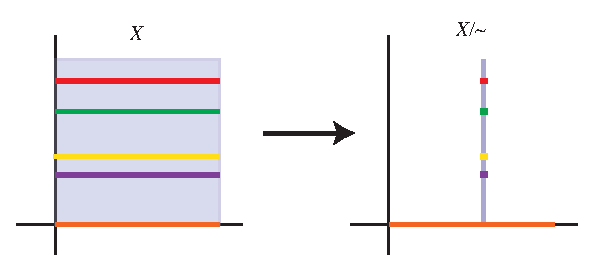
\includegraphics[width=280pt]{images/hausdorffness/IxInonexample}\]
	Points of the same color are identified. Points on the $x$-axis are not separable, so this is a Hausdorff space $X$ and an equivalence relation $\sim$ such that $X/\sim$ is not Hausdorff. 
\end{example}
\begin{example}
	Let $X=\R,$ and set $x \sim y$ if and only if $x=y$ or $x,y>0.$ 
	
	\[
	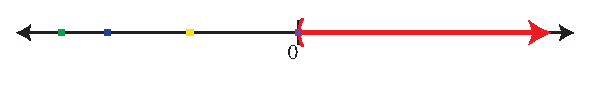
\includegraphics[width=360pt]{images/hausdorffness/r_nonexample}\]
	
	Let $p>0.$ Then $[p],[0]\in X/\sim$. Let $U \subseteq X/\sim$ be an open set containing $[0].$ We claim that $[p]\in U$. To see why, note that $\pi^{-1}(U)$ is an open subset of $\R$ containing $0$. Hence, there exists $q \in \pi^{-1}(U)$ such that $q>0.$ Therefore, $q \sim p \Rightarrow [q]=[p]\in U$, and $X/\sim$ is not Hausdorff. 
\end{example}

Note: this proves that the continuous images of a Hausdorff space need not be Hausdorff! 
